\documentclass[tikz, border=10pt]{standalone}
\usepackage{iftex}
\ifluatex
  \usepackage{fontspec}
  \usepackage{unicode-math}
  \setmainfont{Fira Sans}
  \setmonofont{Fira Mono}
  \setmathfont{Fira Math}
  % Fallback only for set-difference glyphs missing in Fira Math.
  \setmathfont{STIX Two Math}[range={"29F5,"2216}]
\else
  \usepackage[T1]{fontenc}
  \usepackage{newtxtext}
  \usepackage{newtxmath}
\fi

\usepackage{amsmath}
\usepackage{tikz}
\usetikzlibrary{arrows.meta, positioning, calc}
\tikzset{every node/.style={font=\Large}}

% Theme toggle: set \darkbgfalse for light background preview.
\newif\ifdarkbg
\darkbgtrue
\ifdarkbg
  \colorlet{setoutline}{white}
  \colorlet{setlabel}{white}
  \colorlet{pointcol}{white}
  \colorlet{pointlabel}{green!85!white}
  \colorlet{arrowcol}{cyan!85!white}
\else
  \colorlet{setoutline}{black}
  \colorlet{setlabel}{black}
  \colorlet{pointcol}{black}
  \colorlet{pointlabel}{blue!70!black}
  \colorlet{arrowcol}{blue!70!black}
\fi

\begin{document}
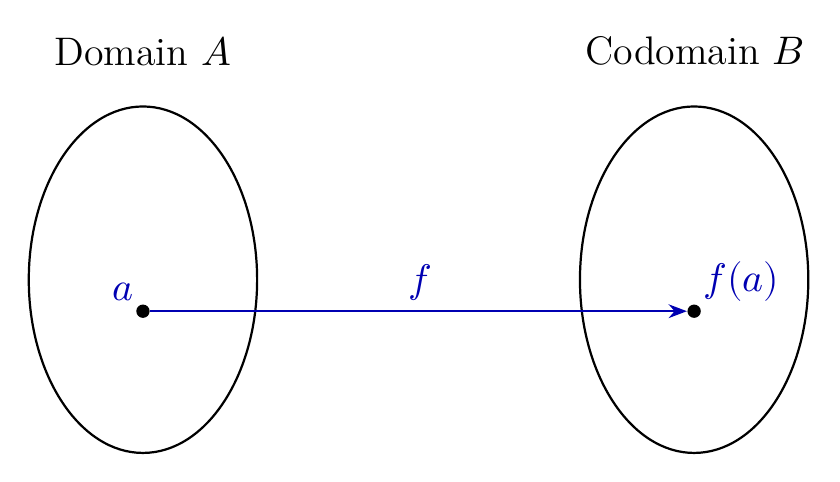
\begin{tikzpicture}[>=Stealth]

% Domain A
\draw[thick, setoutline] (2,0) ellipse [x radius=1.45, y radius=2.2];
\node[text=setlabel] at (2,2.9) {Domain $A$};

% Codomain B
\draw[thick, setoutline] (9,0) ellipse [x radius=1.45, y radius=2.2];
\node[text=setlabel] at (9,2.9) {Codomain $B$};

% Points
\node[circle, fill=pointcol, inner sep=1.7pt] (a1) at (2,-0.4) {};
\node[circle, fill=pointcol, inner sep=1.7pt] (b1) at (9,-0.4) {};
\node[above left, text=pointlabel] at (a1) {$a$};
\node[above right, text=pointlabel] at (b1) {$f(a)$};

% Function arrow
\draw[->, thick, arrowcol] (a1) -- (b1)
  node[midway, above, text=arrowcol] {$f$};

\end{tikzpicture}
\end{document}
